\documentclass[12pt]{article}
\usepackage{geometry}
\usepackage{booktabs}
\usepackage{longtable}
\usepackage{hyperref}
\usepackage{graphicx}
\geometry{margin=2.5cm}
\usepackage{float}

\begin{document}

\section{Essai de différents modèles Huggingface}

\subsection{Préparation et sélection des données}
J'ai pris tous les messages et j'ai gardé ceux annotés, j'ai equilibré le nombre de BULLISH/BEARISH pour l'entrainement et le test.
Les messages ont été modifié pour supprimer toute mention de leur ticker afin de ne pas apprendre sur la popularité des symboles mais bien sur le sens des phrases.
Les tickers considérés sont TSLA, AAPL, AMD, NVDA, GOOGL, META : je les ai choisi car les utilisateurs qui parlent de l'un vont parler des autres et cela est intéressant pour pouvoir mieux généraliser lorsque l'on veut créer un embedding utlisateur pour rajouter du contexte à la prédiction.


\begin{longtable}{lccccc}
\caption{Modèle utilisé / nombre de messages utilisés / précision sur dataset équilibré} \\
\toprule
\textbf{modèle utilisé} & 10k & 100k & 400k & 1M & 2M \\
\midrule
microsoft/mpnet-base & 71.8\% & 70.5\% & 83.0\% & coll. & 81.7\% \\
distilroberta-base & 69.1\% & 77.7\% & 77.9\% & -- & -- \\
albert-large-v2 & 70.5\% & 72.6\% & -- & -- & -- \\
google/electra-base-discriminator & 71.8\% & 78.9\% & 79.8\% & 81.3\% & 82.4\% \\
google/electra-small-discriminator & 61.1\% & 72.9\% & 72.8\% & -- & -- \\
cardiffnlp/twitter-roberta-base-sentiment & 70.5\% & 80.7\% & 82.2\% & 82.3\% & 82.9\% \\
cardiffnlp/twitter-roberta-base & 71.8\% & 78.5\% & 80.8\% & 79.6\% & 82.9\% \\
yiyanghkust/finbert-tone & 66.4\% & 75.4\% & 77.0\% & 79.3\% & 82.0\% \\
\bottomrule
\caption*{\small Après équilibrage, environ 80\% des messages sont supprimés (donc 100\_000 correspond a environ 20\_000 réellement utilisés)}
\end{longtable}


On remarque que twitter-roberta-base-sentiment est rapidement bon et qu'il devient le meilleur avec un gros entrainement. Le modèle est de taille moyenne.
Je l'ai donc choisi pour poursuivre mon étude.

Certains tweets sont plus facilement catégorisable : notamenent les tweets plus long.


\begin{table}[h]
\caption{Précision sur dataset équilibré en fonction du nombre T de tokens du message}
\centering
\begin{tabular}{cccc}
\toprule
T$\le$32 & 32$<$T$\le$64 & 64$<$T$\le$128 & 128$<$T$\le$256 \\
\midrule
82.5\% & 88.0\% & 91.9\% & 91.1\% \\
\bottomrule
\end{tabular}

\vspace{2mm}
{\centering \small Entrainement sur 1500000 messages et test sur 15000 tweets.\par}

\end{table}


J'ai découvert que le fait de passer un liste de token bornée permet un gain de perfomances gpu énorme et un usage moindre de la mémoire.
J'ai donc adapté le process pour entrainer par tranche : d'abord les tweets de moins de 32 puis entre 32 et 64 (moins nombreux) etc.
J'ai trouvé aussi que pour interpréter un embedding généré, le mieux etait de récupérer un layer du modèle plutot que de faire un réseau complétement
connecté.
Une tête simple est généralement plus performante.
Il ne faut surtout pas entrainer le transformer sur plus de deux époques sinon il apprend par coeur : on voit la loss diminuer mais la performance 
n'augmente pas (voir diminue). La solution est d'utiliser beaucoup de messages (ce qui est assez lent à traiter).

\section{Ajout de contexte pour améliorer la prédiction}

J'utilise 1500000 messages pour l'entrainnement (pour des raisons de RAM)

2 idées :
\begin{itemize}

    \item Certains utilisateurs ont une façon bien à eux de s'exprimer et il est intéressant donner un descriptif de l'utilisateur : on peut le représenter comme la moyenne de ses embeddings précédent (tout tickers confondu). L'embedding ainsi obtenu est ramené sur un latent de dimension 2 pour généralisation.
    
    \item Certains messages sont neutres et viennent en réponse à d'autres ; certains sont ambigus : Une première idée consiste à prendre en compte les précédents messages pour voir si on peut clarifier ces tweets : chaque tweet produit un embedding et on créé une colonne previous qui est une moyenne pondérée des précédent tweet avec un mécanisme d'attention sommaire :\\
    \texttt{current\_mean := (previous\_embedding + current\_mean) / 2}\\
    l'embedding ainsi obtenu est également ramené sur un latent de dimension 2 pour généralisation.

\end{itemize}

\begin{figure}[h]
\centering
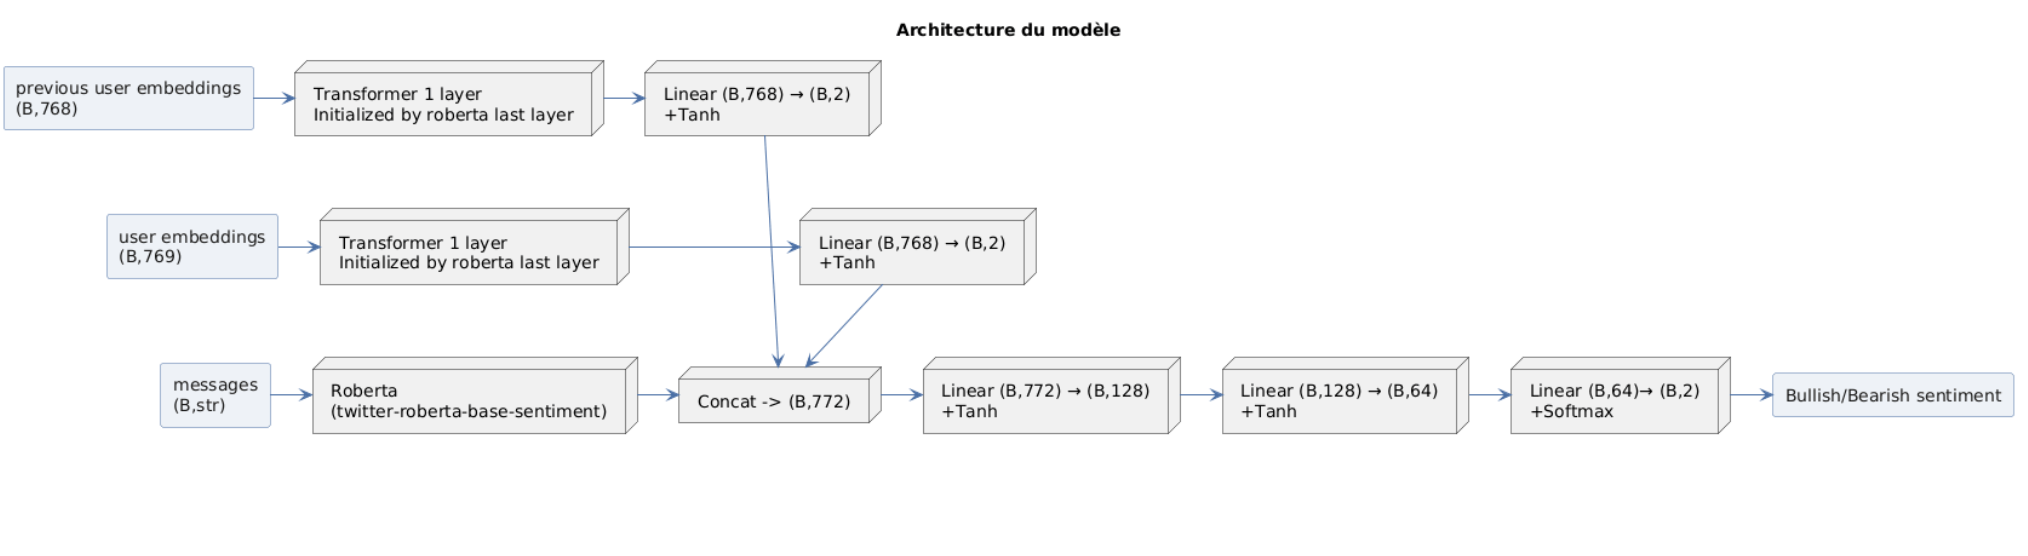
\includegraphics[width=1.1\textwidth]{schéma.png}
\caption{Schéma général du modèle avec previous embedding et user embedding}
\end{figure}



\begin{table}[H]
\centering
\caption{Performances évaluées sur 60000 tweets}
\begin{tabular}{lc}
\toprule
Modèle utilisé & performances \\
\midrule
roberta + simple tete de classification & 83.14\% \\
ajout du user embedding & 88.24\% \\
ajout du previous embedding & 86.19\% \\
ajout du previous embedding et du user embedding & 88.72\% \\
\bottomrule
\end{tabular}
\end{table}

Dans le cas previous embedding + user embedding, on remarque un gain significatif pour les petits messages (test sur 15000 tweets) : 

\begin{center}
\begin{tabular}{lcccc}
\toprule
 & T$\le$32 & 32$<$T$\le$64 & 64$<$T$\le$128 & 128$<$T$\le$256 \\
\midrule
roberta + simple tete de classification & 82.5\% & 88.0\% & 91.9\% & 91.1\% \\
ajout du user embedding & 88.9\% & 91.4\% & 89.4\% & 91.1\% \\
ajout du previous embedding & 86.6\% & 86.7\% & 88.6\% & 90.2\% \\
ajout du previous embedding et du user embedding & 89.1\% & 89.6\% & 88.7\% & 90.3\% \\
\bottomrule
\end{tabular}
\end{center}
\\
Sur les tweets long (qui sont beaucoup moins nombreux), on note une légère baisse de performances avec l'ajout du contexte (T<64) surtout celui du previous embedding (T<32). Mais la performance globale s'améliore car les tweets majoritaires font moins de 32 tokens. Si on prennait les perfs max pour chaque modèle,
on voit que l'on atteindrait les 90\% au global ...

\section{Conclusion}
On peut donc avoir une très bonne prévision des tweets en prennant en compte la personnalité de l'utilisateur et ses précédent tweets, et ce, même avec des tweets ambigus. 

\section{Points qui reste en suspend}

\begin{itemize}
\item  Il serait intéressant de fournir le nombre de tokens au modèle pour que celui-ci apprenne à faire d'avantage confiance à l'embedding de l'utilisateur
lorsque celui-ci a suffisament de tokens (et donc moins utiliser les infos du contexte) : Avec un peu plus de temps sur ce projet, cela aurait été la 
prochaine étape.
\item  On pourrait essayer d'améliorer la prise en compte des messages précédents : régler mieux l'attention
\item  Gérer les tweets qui sont des réponses, rajouter le tweet initial en contexte
\item  Il serait intéressant de voir si un user embedding reste crédible longtemps si on ne fait de mise à jour 
\item  Les hyper paramètres du réseau que j'ai créé doivent pouvoir être optimisés 
\item  Il arrive parfois qu'un modèle "collapse" en début d'entrainement (même le modèle le plus simple avec 1 tête de classification) :
Dans ce cas la, je relance et le shuffle fait l'affaire : je pense que pour stabiliser l'apprentissage il serait peut être intéressant de le
nourrir au début avec des tweets qui sont certainnement non ambigu.
\end{itemize}

\section{Repository github publique}

\url{https://github.com/matthieubaucher/projet_NLP}

Pour le télécharger directement : 

\texttt{git@github.com:matthieubaucher/projet_NLP.git}

\end{document}
